%% \documentclass[11pt]{article}
%%\usepackage{beamerarticle}
\documentclass[extsize,handout,10pt]{beamer}\usepackage[]{graphicx}\usepackage[]{color}
% maxwidth is the original width if it is less than linewidth
% otherwise use linewidth (to make sure the graphics do not exceed the margin)
\makeatletter
\def\maxwidth{ %
  \ifdim\Gin@nat@width>\linewidth
    \linewidth
  \else
    \Gin@nat@width
  \fi
}
\makeatother

\definecolor{fgcolor}{rgb}{0.251, 0.251, 0.251}
\newcommand{\hlnum}[1]{\textcolor[rgb]{0.502,0.086,1}{#1}}%
\newcommand{\hlstr}[1]{\textcolor[rgb]{1,0.4,0.2}{#1}}%
\newcommand{\hlcom}[1]{\textcolor[rgb]{1,0.251,0.502}{#1}}%
\newcommand{\hlopt}[1]{\textcolor[rgb]{0.251,0.251,0.251}{#1}}%
\newcommand{\hlstd}[1]{\textcolor[rgb]{0.251,0.251,0.251}{#1}}%
\newcommand{\hlkwa}[1]{\textcolor[rgb]{0.941,0.188,0.816}{#1}}%
\newcommand{\hlkwb}[1]{\textcolor[rgb]{0,0.439,0.902}{#1}}%
\newcommand{\hlkwc}[1]{\textcolor[rgb]{0.188,0.941,0.314}{#1}}%
\newcommand{\hlkwd}[1]{\textcolor[rgb]{0.69,0.188,0.941}{#1}}%
\let\hlipl\hlkwb

\usepackage{framed}
\makeatletter
\newenvironment{kframe}{%
 \def\at@end@of@kframe{}%
 \ifinner\ifhmode%
  \def\at@end@of@kframe{\end{minipage}}%
  \begin{minipage}{\columnwidth}%
 \fi\fi%
 \def\FrameCommand##1{\hskip\@totalleftmargin \hskip-\fboxsep
 \colorbox{shadecolor}{##1}\hskip-\fboxsep
     % There is no \\@totalrightmargin, so:
     \hskip-\linewidth \hskip-\@totalleftmargin \hskip\columnwidth}%
 \MakeFramed {\advance\hsize-\width
   \@totalleftmargin\z@ \linewidth\hsize
   \@setminipage}}%
 {\par\unskip\endMakeFramed%
 \at@end@of@kframe}
\makeatother

\definecolor{shadecolor}{rgb}{.97, .97, .97}
\definecolor{messagecolor}{rgb}{0, 0, 0}
\definecolor{warningcolor}{rgb}{1, 0, 1}
\definecolor{errorcolor}{rgb}{1, 0, 0}
\newenvironment{knitrout}{}{} % an empty environment to be redefined in TeX

\usepackage{alltt}
\usepackage{preambBeamer} %%preambBeamer for presentation (no hyperref, etc.)
\usepackage{texab} %%Abkürzungen

\mode<article>{\usepackage{}}
\mode<presentation>{\usetheme{} \usecolortheme{}}
\setbeamertemplate{footline}[frame number]





%\pgfpagesuselayout{4 on 1}[a4paper,border shrink=5mm, landscape]
\bibliographystyle{alpha}



\title{Beschreibende Statistik}
%\subtitle{Beschreibende Statistik mit \textsf{R}}
\author{André Meichtry\thanks{\WebConsult}}
%\institute{\G \\ \ZHAW}
\date{2019}
%\titlegraphic{\includegraphics[width=.2\textwidth]{/home/meichtry/BERATUNG/zhawD.jpg}}
\IfFileExists{upquote.sty}{\usepackage{upquote}}{}
\begin{document}

\selectlanguage{english}



\maketitle
\frame{\tableofcontents}





\section{Introduction}



\begin{frame}
  \frametitle{Statistics}
  \begin{itemize}
  \item \alert{Descriptive} statistics
    \begin{itemize}
    \item describe data
    \end{itemize}
  \item \alert{Inferential} statistics
    \begin{itemize}
    \item what is the best guess of the truth, given some data? $\rightarrow${
        point estimation}
    \item what is a range of plausible truths, given the data?
      $\rightarrow${  estimation, confidence intervals}
    \item is a specific truth plausible? $\rightarrow${ hypothesis testing}
    \end{itemize}
  \end{itemize}
\end{frame}


\section{Univariate data}

\begin{frame}
  \frametitle{Terminology}
  \begin{itemize}
  \item \alert{statistical unit}: one member of a set of entities
    being studied
  \item \alert{variable}: quantified aspect of the statistical unit
  \item \alert{population}: arbitrary defined set of units (with in-
    and exclusion criteria)
  \item \alert{sample}: subset of the population, in the ideal case,
    randomly chosen from the population
  \end{itemize}
\end{frame}



    
    



\begin{frame}[containsverbatim]
  \frametitle{Read in data \texttt{read.table()}}
  Example data \emph{stroke.csv}
  \begin{itemize}
    \scriptsize
  \item 
\begin{knitrout}\tiny
\definecolor{shadecolor}{rgb}{0.973, 0.973, 0.973}\color{fgcolor}\begin{kframe}
\begin{alltt}
\hlkwd{rm}\hlstd{(}\hlkwc{list}\hlstd{=}\hlkwd{ls}\hlstd{())}
\hlstd{mydata}  \hlkwb{<-}  \hlkwd{read.csv}\hlstd{(}\hlstr{"https://raw.githubusercontent.com/mcdr65/StatsRsource/master/Data/stroke.csv"}\hlstd{)}
\end{alltt}
\end{kframe}
\end{knitrout}

\begin{knitrout}\tiny
\definecolor{shadecolor}{rgb}{0.973, 0.973, 0.973}\color{fgcolor}\begin{kframe}
\begin{alltt}
\hlkwd{head}\hlstd{(mydata)}
\end{alltt}
\begin{verbatim}
##     SEX AGE DGN COMA DIAB MINF HAN
## 1   man  76 INF   no   no  yes  no
## 2   man  58 INF   no   no   no  no
## 3   man  74 INF   no   no  yes yes
## 4 women  77 ICH   no  yes   no yes
## 5 women  76 INF   no  yes   no yes
## 6   man  48 ICH  yes   no   no yes
\end{verbatim}
\end{kframe}
\end{knitrout}

  \normalsize
  \item for \texttt{Excel}-data: Look at helpfiles
    \alert{\texttt{?read.table}} and \alert{\texttt{?read.csv}} for further
    information
  \item \alert{see preparation exercise!!} 
  \end{itemize}
\end{frame}



\begin{frame}[containsverbatim]
  \frametitle{Look at data}
  \small
Let us look at a simple dataset
    (\alert{\texttt{chickwts}}) available in the \textsf{R} environment:
    
\begin{knitrout}\tiny
\definecolor{shadecolor}{rgb}{0.973, 0.973, 0.973}\color{fgcolor}\begin{kframe}
\begin{alltt}
\hlkwd{head}\hlstd{(chickwts)} \hlcom{##only the first observations}
\end{alltt}
\begin{verbatim}
##   weight      feed
## 1    179 horsebean
## 2    160 horsebean
## 3    136 horsebean
## 4    227 horsebean
## 5    217 horsebean
## 6    168 horsebean
\end{verbatim}
\end{kframe}
\end{knitrout}
\end{frame}


\begin{frame}[containsverbatim]
  \frametitle{\texttt{help()}}
\alert{Very important: help files for \textsf{R}-functions}. 

For example, the help for the function \texttt{median}

\begin{knitrout}\tiny
\definecolor{shadecolor}{rgb}{0.973, 0.973, 0.973}\color{fgcolor}\begin{kframe}
\begin{alltt}
\hlkwd{help}\hlstd{(median)}
\hlcom{## or ?median}
\end{alltt}
\end{kframe}
\end{knitrout}

\end{frame}


\begin{frame}[containsverbatim]
    \frametitle{Look at object, \texttt{str()}}
  look at the \alert{structure} of \textsf{R}-objects
  \small
  
\begin{knitrout}\tiny
\definecolor{shadecolor}{rgb}{0.973, 0.973, 0.973}\color{fgcolor}\begin{kframe}
\begin{alltt}
\hlkwd{str}\hlstd{(chickwts)}
\end{alltt}
\begin{verbatim}
## 'data.frame':	71 obs. of  2 variables:
##  $ weight: num  179 160 136 227 217 168 108 124 143 140 ...
##  $ feed  : Factor w/ 6 levels "casein","horsebean",..: 2 2 2 2 2 2 2 2 2 2 ...
\end{verbatim}
\end{kframe}
\end{knitrout}

\end{frame}




\begin{frame}
  \frametitle{Measurement scales}
  the \alert{scale} of measurement depends on the \alert{preserved
    property} during the mapping of the \alert{empirical world} into
  the \alert{numerical world}:
  \begin{table}[h]
    \centering
    \begin{tabular}{llll}
      \alert{scale}&\alert{preserves}&\alert{example}&\alert{operations}\\\hline
      nominal&categories&gender&$=,\neq$\\
      ordinal&order& independence score&$\leq,\geq$\\
      interval&equidistance&celcius&$+,-$\\
      ratio&ratios& kelvin&$\cdot,/$\\
    \end{tabular}
    \caption[measurement scales]{measurement scales}
    \label{tab:Skalenniveaus}
  \end{table}
\end{frame}


\begin{frame}[containsverbatim]
  \frametitle{\textsf{R}, creation of new variables}

\begin{knitrout}\tiny
\definecolor{shadecolor}{rgb}{0.973, 0.973, 0.973}\color{fgcolor}\begin{kframe}
\begin{alltt}
\hlcom{##weight in kilograms}
\hlstd{chickwts}\hlopt{$}\hlstd{weightkg} \hlkwb{<-} \hlstd{chickwts}\hlopt{$}\hlstd{weight}\hlopt{/}\hlnum{1000}
\hlkwd{str}\hlstd{(chickwts)}
\end{alltt}
\begin{verbatim}
## 'data.frame':	71 obs. of  3 variables:
##  $ weight  : num  179 160 136 227 217 168 108 124 143 140 ...
##  $ feed    : Factor w/ 6 levels "casein","horsebean",..: 2 2 2 2 2 2 2 2 2 2 ...
##  $ weightkg: num  0.179 0.16 0.136 0.227 0.217 0.168 0.108 0.124 0.143 0.14 ...
\end{verbatim}
\end{kframe}
\end{knitrout}
\end{frame}  


\begin{frame}[containsverbatim]
  \frametitle{Look at first observations, \texttt{head()}}
\begin{knitrout}\tiny
\definecolor{shadecolor}{rgb}{0.973, 0.973, 0.973}\color{fgcolor}\begin{kframe}
\begin{alltt}
\hlkwd{head}\hlstd{(chickwts)}
\end{alltt}
\begin{verbatim}
##   weight      feed weightkg
## 1    179 horsebean    0.179
## 2    160 horsebean    0.160
## 3    136 horsebean    0.136
## 4    227 horsebean    0.227
## 5    217 horsebean    0.217
## 6    168 horsebean    0.168
\end{verbatim}
\end{kframe}
\end{knitrout}
\end{frame}



\begin{frame}
  \frametitle{Sample}
  \begin{itemize}
  \item $n$ \alert{observations} of a \alert{random variable} $X$
    \begin{equation*}
      \label{eq:Realisierung von Stichprobenvariablen}
      X_1=x_1,\quad X_2=x_2,\quad\ldots,\quad X_n=x_n.
    \end{equation*}
  \item $n$: sample size
  \item<2-> $X$: random quantity which is observed $n$-times
  \item<3-> $X_1,X_2,\ldots,X_{n}$
    constitutes a \alert{sample}
  \item<5-> $X$ is \alert{random}, because each unit is viewed as
    randomly chosen unit from
    the population
  \item How many observations has \alert{\texttt{chickwts}}, how many variables
    has \alert{\texttt{chickwts}}
  \end{itemize}
\end{frame}
    

\begin{frame}
  \frametitle{Frequencies}
  \begin{itemize}
  \item<1-> \alert{absolute frequency} $f$ [$f$: "`frequency"']: The
    \structure{number} of observations of a \structure{specific value}
    on the variable $X$
  \item \alert{relative frequency} $f_{rel}$: The
    \structure{proportion} of observations that have a
    \structure{specific value} on the variable $X$
  \item<2-> \alert{absolute cumulative frequency}: $F$: The
    \structure{number} of observations that are \structure{smaller or
      equal} ($\leq$) than a specific value on the variable $X$
  \item \alert{relative cumulative frequency} $F_{rel}$: The
    \structure{proportion} of observations that are \structure{smaller
      or equal} ($\leq$) than a specific value on the variable $X$
  \end{itemize}
\end{frame}




\begin{frame}[containsverbatim]
  \frametitle{Frequency distribution, histogram, \texttt{hist()}}

\begin{knitrout}\tiny
\definecolor{shadecolor}{rgb}{0.973, 0.973, 0.973}\color{fgcolor}\begin{kframe}
\begin{alltt}
\hlkwd{hist}\hlstd{(chickwts}\hlopt{$}\hlstd{weightkg,}\hlkwc{xlab}\hlstd{=}\hlstr{"Gewicht(kg)"}\hlstd{,}\hlkwc{freq}\hlstd{=}\hlnum{FALSE}\hlstd{)}
\end{alltt}
\end{kframe}

{\centering 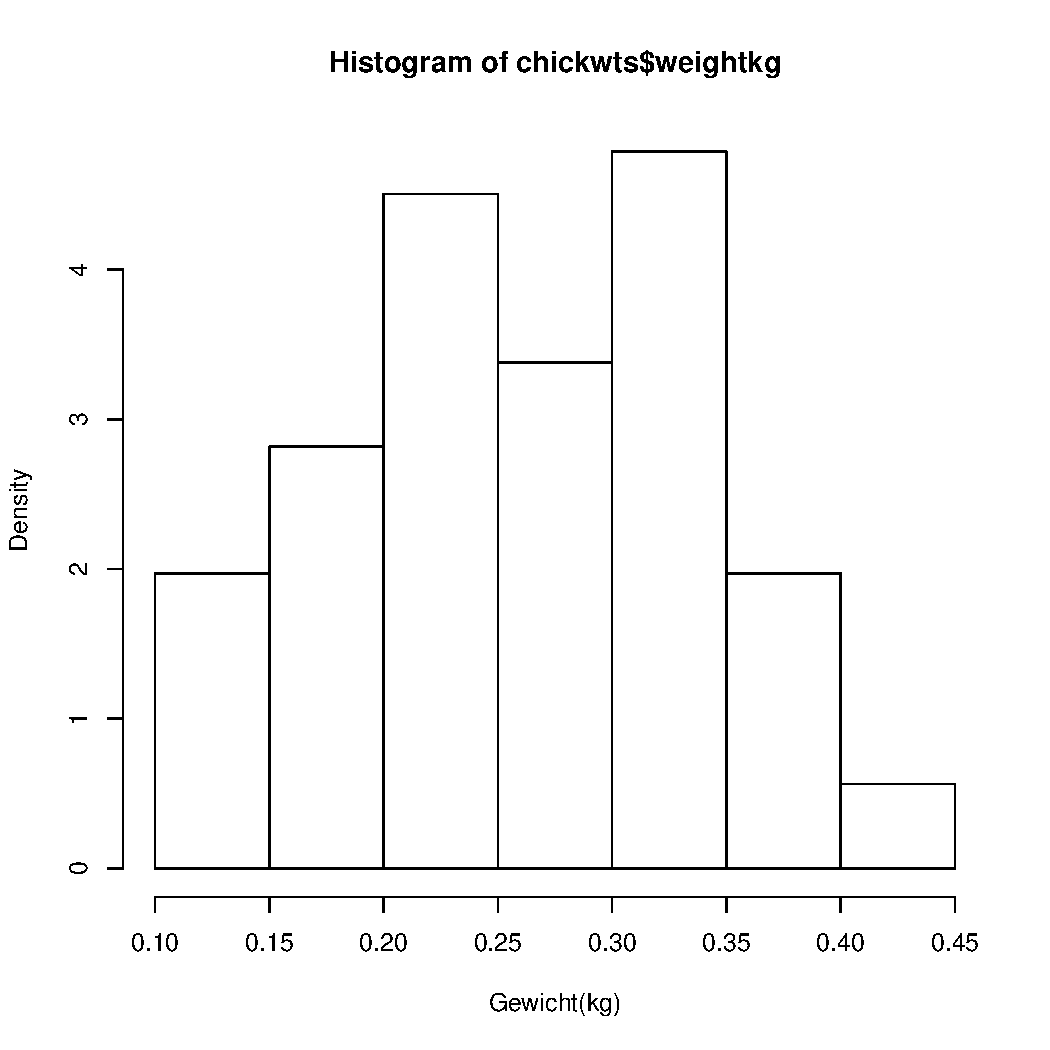
\includegraphics[width=.49\linewidth]{figures/unnamed-chunk-10-1} 

}



\end{knitrout}

\end{frame}



\begin{frame}[containsverbatim]
  \frametitle{Empirical cumulative distribution, \texttt{ecdf()}}
\begin{knitrout}\tiny
\definecolor{shadecolor}{rgb}{0.973, 0.973, 0.973}\color{fgcolor}\begin{kframe}
\begin{alltt}
\hlstd{cumfreq}\hlkwb{<-}\hlkwd{ecdf}\hlstd{(chickwts}\hlopt{$}\hlstd{weightkg)}
\hlkwd{plot}\hlstd{(cumfreq,}\hlkwc{xlab}\hlstd{=}\hlstr{"weight"}\hlstd{,}\hlkwc{main}\hlstd{=}\hlstr{"cumul.freq."}\hlstd{)}
\end{alltt}
\end{kframe}

{\centering 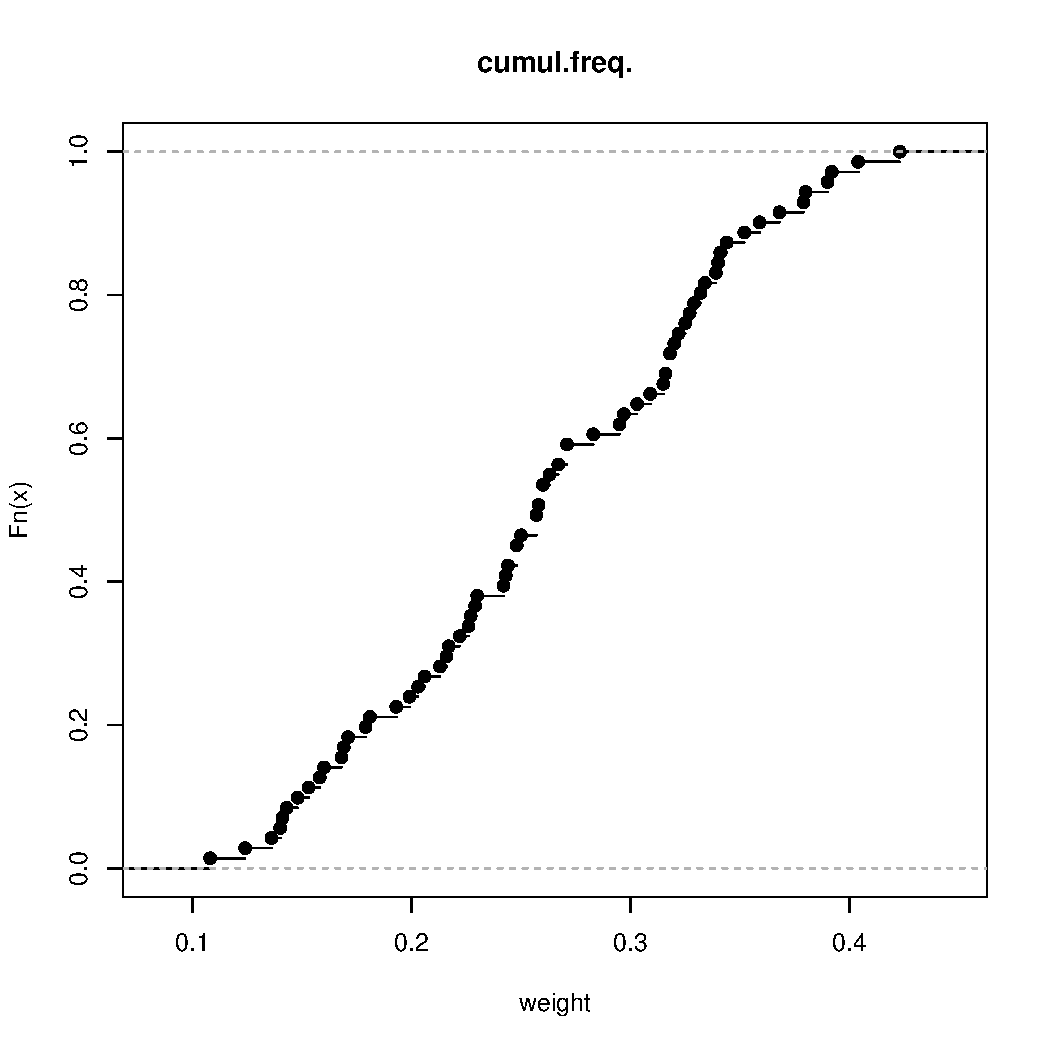
\includegraphics[width=.49\linewidth]{figures/unnamed-chunk-11-1} 

}



\end{knitrout}

\end{frame}

\begin{frame}[containsverbatim]
  \frametitle{Did we understand \texttt{ecdf()}?}
\begin{knitrout}\tiny
\definecolor{shadecolor}{rgb}{0.973, 0.973, 0.973}\color{fgcolor}\begin{kframe}
\begin{alltt}
\hlkwd{cumfreq}\hlstd{(}\hlkwd{max}\hlstd{(chickwts}\hlopt{$}\hlstd{weightkg))}
\end{alltt}
\begin{verbatim}
## [1] 1
\end{verbatim}
\begin{alltt}
\hlkwd{cumfreq}\hlstd{(}\hlkwd{median}\hlstd{(chickwts}\hlopt{$}\hlstd{weightkg))}
\end{alltt}
\begin{verbatim}
## [1] 0.507
\end{verbatim}
\end{kframe}
\end{knitrout}
\end{frame}


\begin{frame}[containsverbatim]
  \frametitle{\texttt{summary()}}

\begin{knitrout}\tiny
\definecolor{shadecolor}{rgb}{0.973, 0.973, 0.973}\color{fgcolor}\begin{kframe}
\begin{alltt}
\hlkwd{summary}\hlstd{(chickwts)}
\end{alltt}
\begin{verbatim}
##      weight           feed       weightkg    
##  Min.   :108   casein   :12   Min.   :0.108  
##  1st Qu.:204   horsebean:10   1st Qu.:0.204  
##  Median :258   linseed  :12   Median :0.258  
##  Mean   :261   meatmeal :11   Mean   :0.261  
##  3rd Qu.:324   soybean  :14   3rd Qu.:0.324  
##  Max.   :423   sunflower:12   Max.   :0.423
\end{verbatim}
\end{kframe}
\end{knitrout}
\end{frame}



\begin{frame}[containsverbatim]
  \frametitle{\texttt{boxplot()}}
\begin{knitrout}\tiny
\definecolor{shadecolor}{rgb}{0.973, 0.973, 0.973}\color{fgcolor}\begin{kframe}
\begin{alltt}
\hlkwd{boxplot}\hlstd{(weight}\hlopt{~}\hlstd{feed,}\hlkwc{data}\hlstd{=chickwts,}
        \hlkwc{ylab}\hlstd{=}\hlstr{"weight"}\hlstd{,}\hlkwc{xlab}\hlstd{=}\hlstr{"feed"}\hlstd{,}\hlkwc{las}\hlstd{=}\hlnum{2}\hlstd{)}
\end{alltt}
\end{kframe}

{\centering 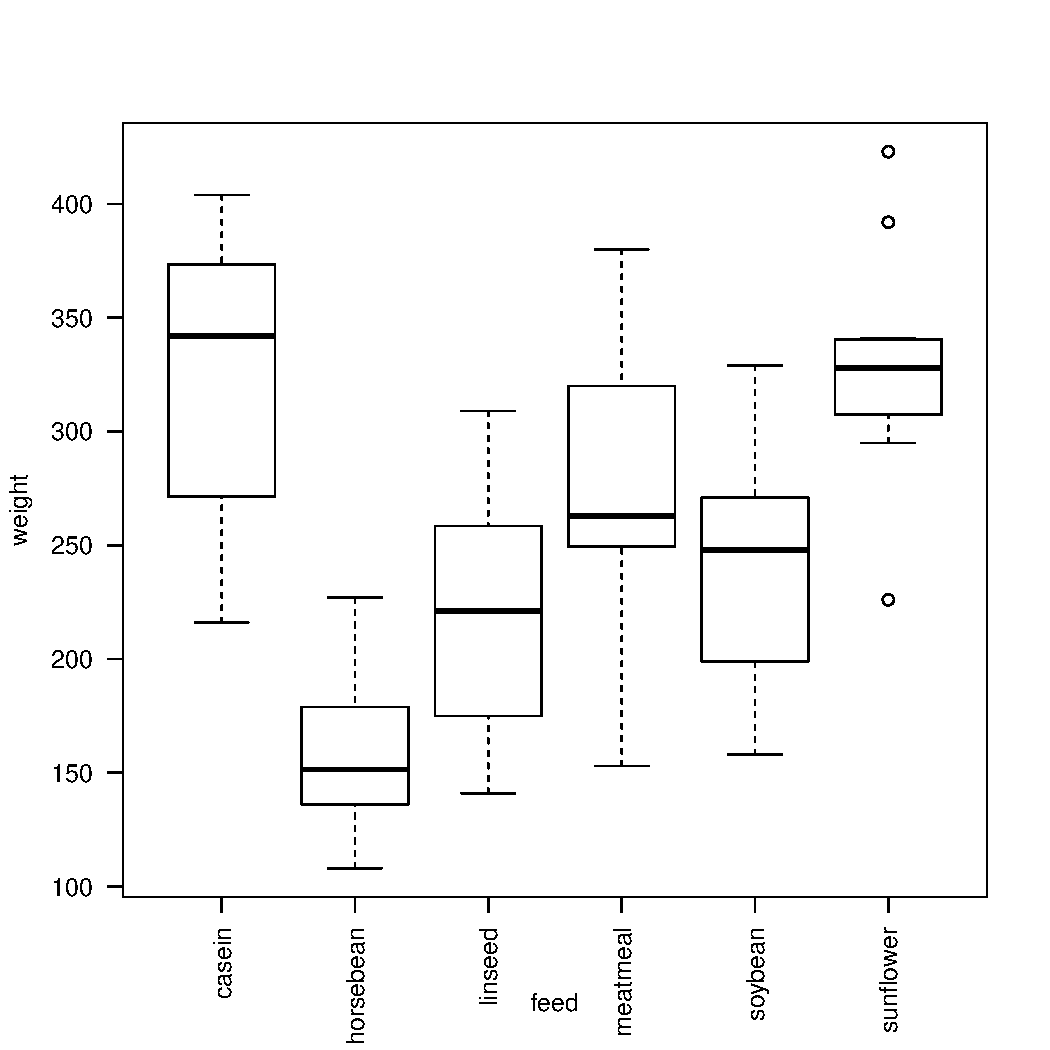
\includegraphics[width=.49\linewidth]{figures/unnamed-chunk-14-1} 

}



\end{knitrout}
\end{frame}


\begin{frame}[containsverbatim]
  \frametitle{summary measures of data subsets, \texttt{aggregate()}}
  \small
\begin{knitrout}\tiny
\definecolor{shadecolor}{rgb}{0.973, 0.973, 0.973}\color{fgcolor}\begin{kframe}
\begin{alltt}
\hlkwd{aggregate}\hlstd{(chickwts}\hlopt{$}\hlstd{weightkg,}\hlkwc{by}\hlstd{=}\hlkwd{list}\hlstd{(chickwts}\hlopt{$}\hlstd{feed),}\hlkwc{FUN}\hlstd{=}\hlstr{"summary"}\hlstd{)}
\end{alltt}
\begin{verbatim}
##     Group.1 x.Min. x.1st Qu. x.Median x.Mean x.3rd Qu. x.Max.
## 1    casein  0.216     0.277    0.342  0.324     0.371  0.404
## 2 horsebean  0.108     0.137    0.151  0.160     0.176  0.227
## 3   linseed  0.141     0.178    0.221  0.219     0.258  0.309
## 4  meatmeal  0.153     0.249    0.263  0.277     0.320  0.380
## 5   soybean  0.158     0.207    0.248  0.246     0.270  0.329
## 6 sunflower  0.226     0.313    0.328  0.329     0.340  0.423
\end{verbatim}
\end{kframe}
\end{knitrout}
\end{frame}

\begin{frame}[containsverbatim]
  \frametitle{\texttt{aggregate()}}
  \small
\begin{knitrout}\tiny
\definecolor{shadecolor}{rgb}{0.973, 0.973, 0.973}\color{fgcolor}\begin{kframe}
\begin{alltt}
\hlkwd{aggregate}\hlstd{(chickwts}\hlopt{$}\hlstd{weight,}\hlkwc{by}\hlstd{=}\hlkwd{list}\hlstd{(chickwts}\hlopt{$}\hlstd{feed),}\hlkwc{FUN}\hlstd{=}\hlstr{"quantile"}\hlstd{)}
\end{alltt}
\begin{verbatim}
##     Group.1 x.0% x.25% x.50% x.75% x.100%
## 1    casein  216   277   342   371    404
## 2 horsebean  108   137   152   176    227
## 3   linseed  141   178   221   258    309
## 4  meatmeal  153   250   263   320    380
## 5   soybean  158   207   248   270    329
## 6 sunflower  226   313   328   340    423
\end{verbatim}
\end{kframe}
\end{knitrout}
\end{frame}


\begin{frame}[containsverbatim]
  \frametitle{Summary measures of data subsets, \texttt{split()}}
  \small
\begin{knitrout}\tiny
\definecolor{shadecolor}{rgb}{0.973, 0.973, 0.973}\color{fgcolor}\begin{kframe}
\begin{alltt}
\hlstd{subgr} \hlkwb{<-} \hlkwd{split}\hlstd{(chickwts[,}\hlkwd{c}\hlstd{(}\hlnum{1}\hlstd{,}\hlnum{3}\hlstd{)],}\hlkwc{f}\hlstd{=chickwts}\hlopt{$}\hlstd{feed)}
\hlkwd{lapply}\hlstd{(subgr,summary)}
\end{alltt}
\begin{verbatim}
## $casein
##      weight       weightkg    
##  Min.   :216   Min.   :0.216  
##  1st Qu.:277   1st Qu.:0.277  
##  Median :342   Median :0.342  
##  Mean   :324   Mean   :0.324  
##  3rd Qu.:371   3rd Qu.:0.371  
##  Max.   :404   Max.   :0.404  
## 
## $horsebean
##      weight       weightkg    
##  Min.   :108   Min.   :0.108  
##  1st Qu.:137   1st Qu.:0.137  
##  Median :152   Median :0.151  
##  Mean   :160   Mean   :0.160  
##  3rd Qu.:176   3rd Qu.:0.176  
##  Max.   :227   Max.   :0.227  
## 
## $linseed
##      weight       weightkg    
##  Min.   :141   Min.   :0.141  
##  1st Qu.:178   1st Qu.:0.178  
##  Median :221   Median :0.221  
##  Mean   :219   Mean   :0.219  
##  3rd Qu.:258   3rd Qu.:0.258  
##  Max.   :309   Max.   :0.309  
## 
## $meatmeal
##      weight       weightkg    
##  Min.   :153   Min.   :0.153  
##  1st Qu.:250   1st Qu.:0.250  
##  Median :263   Median :0.263  
##  Mean   :277   Mean   :0.277  
##  3rd Qu.:320   3rd Qu.:0.320  
##  Max.   :380   Max.   :0.380  
## 
## $soybean
##      weight       weightkg    
##  Min.   :158   Min.   :0.158  
##  1st Qu.:207   1st Qu.:0.207  
##  Median :248   Median :0.248  
##  Mean   :246   Mean   :0.246  
##  3rd Qu.:270   3rd Qu.:0.270  
##  Max.   :329   Max.   :0.329  
## 
## $sunflower
##      weight       weightkg    
##  Min.   :226   Min.   :0.226  
##  1st Qu.:313   1st Qu.:0.313  
##  Median :328   Median :0.328  
##  Mean   :329   Mean   :0.329  
##  3rd Qu.:340   3rd Qu.:0.340  
##  Max.   :423   Max.   :0.423
\end{verbatim}
\end{kframe}
\end{knitrout}
\end{frame}


\begin{frame}[containsverbatim]
  \frametitle{Kreuztabellen, \texttt{table()}}  

\small

\begin{knitrout}\tiny
\definecolor{shadecolor}{rgb}{0.973, 0.973, 0.973}\color{fgcolor}\begin{kframe}
\begin{alltt}
\hlkwd{head}\hlstd{(mydata)}
\end{alltt}
\begin{verbatim}
##     SEX AGE DGN COMA DIAB MINF HAN
## 1   man  76 INF   no   no  yes  no
## 2   man  58 INF   no   no   no  no
## 3   man  74 INF   no   no  yes yes
## 4 women  77 ICH   no  yes   no yes
## 5 women  76 INF   no  yes   no yes
## 6   man  48 ICH  yes   no   no yes
\end{verbatim}
\begin{alltt}
\hlkwd{table}\hlstd{(mydata[,}\hlkwd{c}\hlstd{(}\hlnum{1}\hlstd{,}\hlnum{5}\hlstd{)])}
\end{alltt}
\begin{verbatim}
##        DIAB
## SEX      no yes
##   man   291  28
##   women 441  69
\end{verbatim}
\end{kframe}
\end{knitrout}
\end{frame}




\begin{frame}
  \frametitle{Boxplot}
  \begin{itemize}
  \item<1-> median: \alert{$0.5$-quantile}
  \item<2-> the box goes from the \alert{$0.25$-quantile} to the
    \alert{$0.75$-quantile}. This distance is the interquartile range
    (IQR)
  \item<3->the lines go to the value of the data point which lies
    still below of \alert{$0.75$-quantile + 1.5 IQR} resp. above
    \alert{$0.25$-quantiles - 1.5 IQR}
  \end{itemize}
\end{frame}




\begin{frame}[containsverbatim]
  \frametitle{Quantile: \texttt{quantile()}}
\begin{knitrout}\tiny
\definecolor{shadecolor}{rgb}{0.973, 0.973, 0.973}\color{fgcolor}\begin{kframe}
\begin{alltt}
\hlkwd{quantile}\hlstd{(chickwts}\hlopt{$}\hlstd{weightkg)}
\end{alltt}
\begin{verbatim}
##    0%   25%   50%   75%  100% 
## 0.108 0.205 0.258 0.324 0.423
\end{verbatim}
\begin{alltt}
\hlkwd{quantile}\hlstd{(chickwts}\hlopt{$}\hlstd{weightkg,}\hlkwc{prob}\hlstd{=}\hlkwd{c}\hlstd{(}\hlnum{.33}\hlstd{,}\hlnum{.66}\hlstd{))}
\end{alltt}
\begin{verbatim}
##   33%   66% 
## 0.226 0.310
\end{verbatim}
\end{kframe}
\end{knitrout}
\end{frame}

\begin{frame}[containsverbatim]
  \frametitle{\texttt{summary()}}
\begin{knitrout}\tiny
\definecolor{shadecolor}{rgb}{0.973, 0.973, 0.973}\color{fgcolor}\begin{kframe}
\begin{alltt}
\hlkwd{summary}\hlstd{(chickwts)}
\end{alltt}
\begin{verbatim}
##      weight           feed       weightkg    
##  Min.   :108   casein   :12   Min.   :0.108  
##  1st Qu.:204   horsebean:10   1st Qu.:0.204  
##  Median :258   linseed  :12   Median :0.258  
##  Mean   :261   meatmeal :11   Mean   :0.261  
##  3rd Qu.:324   soybean  :14   3rd Qu.:0.324  
##  Max.   :423   sunflower:12   Max.   :0.423
\end{verbatim}
\begin{alltt}
\hlkwd{table}\hlstd{(chickwts}\hlopt{$}\hlstd{feed)}
\end{alltt}
\begin{verbatim}
## 
##    casein horsebean   linseed  meatmeal   soybean sunflower 
##        12        10        12        11        14        12
\end{verbatim}
\end{kframe}
\end{knitrout}

\end{frame}






\begin{frame}
  \frametitle{Measures of central tendency/dispersion}
  \begin{table}[h]
    \centering\small
    \begin{tabular}{lccc}
      \hline
      measure / scale &nominal&ordinal&metric\\
      \hline
      \structure{central tendency}& mode& mode, median &mode, median, mean\\
      \structure{dispersion}&& range, IQR & $s$,$s^2$\\
      \hline
    \end{tabular}
  \end{table}
\end{frame}



\begin{frame}
  \frametitle{mean, \texttt{mean()}}
  \begin{itemize}
  \item<1-> \alert{empirical mean} oder \alert{arithmetic mean}:
    \begin{equation*}
      \bar{x}=\frac{x_1+x_2+...+x_n}{n}=\frac{\sum_{i=1}^n{x_i}}{n}
    \end{equation*}
  \item $\bar{x}$ is the most frequent measure of central tendency
  \item<3-> however, $\bar{x}$ is not a \alert{robust} measure of
    central tendency
  \item when we do not have metric data, the arithmetic mean gives no
    sense
  \end{itemize}
\end{frame}




\begin{frame}
  \frametitle{median, \texttt{median()}}
  \begin{itemize}
  \item<1-> \alert{median}: makes sense if variable $X$ is at least
    ordinal scaled
  \item<2-> to calculate the median, we \alert{order} the values of
    $X$
  \item<3-> the median of an \alert{ordered sample} ($x_{(1)},...,x_{(n)}$) of
    $n$ observations is:
    \begin{equation*}
      \text{median}=
      \begin{cases}
        0.5(x_{(n/2)}+x_{(n/2+1)})& \text{if }n\text{ even}\\x_{((n+1)/2)} &
        \text{if } n\text{ uneven}.
      \end{cases}
    \end{equation*}
  \item<4-> this corresponds to the \alert{percentile} $P50$ or to the
    \alert{quantile} $Q_{.5}$.
  \item the median is more \alert{robust} with respect to extreme
    values than the mean $\bar{x}$
  \end{itemize}
\end{frame}


\begin{frame}[containsverbatim]
  \frametitle{mode}
  \begin{itemize}
  \item the \alert{mode} is the value which has the \alert{maximal
      absolute frequency}
    \begin{equation*}
      \label{eq:2}
      \structure{\text{mode}=\arg \underset{x}{\operatorname{max\,}}f(x)}
    \end{equation*}
  \end{itemize}
there is no \texttt{mode}-function in \textsf{R}. 
\begin{knitrout}\tiny
\definecolor{shadecolor}{rgb}{0.973, 0.973, 0.973}\color{fgcolor}\begin{kframe}
\begin{alltt}
\hlstd{x} \hlkwb{<-} \hlkwd{table}\hlstd{(chickwts}\hlopt{$}\hlstd{feed)}
\hlkwd{names}\hlstd{(x)[}\hlkwd{which.max}\hlstd{(x)]}
\end{alltt}
\begin{verbatim}
## [1] "soybean"
\end{verbatim}
\end{kframe}
\end{knitrout}
  
\end{frame}




\begin{frame}
  \frametitle{Measures of dispersion, \texttt{range(), IQR()}}
  \begin{itemize}
  \item<1-> the \alert{range} is the distance between the maximal and
    the minimal value of a sample: max($X$)-min($X$)
  \item<2-> the \alert{$p$-quantile} ($0 \leq p \leq 1$) or
    \alert{$Q_p$} for a random variable $X$ is that value of $X$ which
    corresponds to $p\cdot{100\%}$ of cumulative frequency. For
    example, the median \alert{is} the $Q_{0.5}$
  \item the \alert{interquartil range (IQR)} is the distance between
    $Q_{.25}$ and $Q_{.75}$. (see boxplot)
  \end{itemize}
\end{frame}


\begin{frame}
  \frametitle{Empirical variance, \texttt{var()}}
  \begin{itemize}
  \item the \alert{sample variance} or \alert{empirical variance} is
    the \alert{mean squared deviation} from the mean of the sample
  \item<2-> the empirical sample variance $s^2$ is therefore given by
      \begin{equation*}
        \structure{s^2=\frac{\sum_{i=1}^n{{(x_i-\bar{x})}^2}}{n-1}}.
        \label{Stichprobenvarianz}
      \end{equation*}
    \end{itemize}
  \end{frame}

 
  \begin{frame}
    \frametitle{Sample standard deviation, \texttt{sd()}}
    \begin{itemize}
    \item<1-> if our variable $X$ was body weight, measured in kg,
      then the sample variance has as a unit kg$^2$
    \item to return to the original scale, we take the square root of
      the variance
    \item this quantity is known as the \alert{sample standard
        deviation} or as the \alert{empirical standard deviation} $s$:
      \begin{equation*}
        \structure{
          s=\sqrt{\frac{\sum_{i=1}^n{{(x_i-\bar{x})}^2}}{n-1}}}
        \label{Standardabweichung}
      \end{equation*}
    \end{itemize}
  \end{frame}



  \begin{frame}[containsverbatim]
    \frametitle{Measures of location and dispersion}
    \scriptsize
\begin{knitrout}\tiny
\definecolor{shadecolor}{rgb}{0.973, 0.973, 0.973}\color{fgcolor}\begin{kframe}
\begin{alltt}
\hlkwd{colMeans}\hlstd{(chickwts[,}\hlkwd{c}\hlstd{(}\hlstr{"weight"}\hlstd{,}\hlstr{"weightkg"}\hlstd{)])}
\end{alltt}
\begin{verbatim}
##   weight weightkg 
##  261.310    0.261
\end{verbatim}
\begin{alltt}
\hlkwd{colMeans}\hlstd{(chickwts[,}\hlkwd{c}\hlstd{(}\hlnum{1}\hlstd{,}\hlnum{3}\hlstd{)])}
\end{alltt}
\begin{verbatim}
##   weight weightkg 
##  261.310    0.261
\end{verbatim}
\begin{alltt}
\hlkwd{sd}\hlstd{(chickwts}\hlopt{$}\hlstd{weight)}
\end{alltt}
\begin{verbatim}
## [1] 78.1
\end{verbatim}
\begin{alltt}
\hlkwd{var}\hlstd{(chickwts}\hlopt{$}\hlstd{weight)}
\end{alltt}
\begin{verbatim}
## [1] 6096
\end{verbatim}
\begin{alltt}
\hlkwd{range}\hlstd{(chickwts}\hlopt{$}\hlstd{weight)}
\end{alltt}
\begin{verbatim}
## [1] 108 423
\end{verbatim}
\begin{alltt}
\hlkwd{IQR}\hlstd{(chickwts}\hlopt{$}\hlstd{weight)}
\end{alltt}
\begin{verbatim}
## [1] 119
\end{verbatim}
\end{kframe}
\end{knitrout}
  \end{frame} 
 
    
   
\begin{frame}[containsverbatim]
  \frametitle{Variable $A$ with $n=200$ observations}
  \begin{itemize}
  \item \texttt{rnorm(n,mu,sigma)} \structure{creates $n$ observations from a normal distribution with
    true mean $\mu$ and true standard deviation $\sigma$}
  \item 

\begin{knitrout}\tiny
\definecolor{shadecolor}{rgb}{0.973, 0.973, 0.973}\color{fgcolor}\begin{kframe}
\begin{alltt}
\hlstd{A} \hlkwb{<-} \hlkwd{rnorm}\hlstd{(}\hlnum{200}\hlstd{,}\hlnum{100}\hlstd{,}\hlnum{20}\hlstd{)}
\end{alltt}
\end{kframe}
\end{knitrout}

\item \structure{TASK}: repeat all we have done so far in univariate
  statistics in \textsf{R} with the variable $A$



\item Why the empirical mean (and the empirical SD) is not exactly
  equal to $\mu=100$ ($\sigma=20$), the \structure{known truth} from simulation 
\item Why do we all have slightly different results?
\end{itemize}
\end{frame}
  
  



  \begin{frame}
    \frametitle{Standardisation}
    \begin{itemize}
    \item<1-> to be able to \alert{compare} deviations from the mean,
      we can normalise these deviations with the standard deviation of
      the sample
    \item<2-> this is the \alert{z-transformation}
      \begin{equation*}
        z_i=\frac{x_i-\bar{x}}{s} \qquad    i=1,...,n.
        \label{zTrans}
      \end{equation*}
    \item<3-> the new variable $Z$ has mean 0 and standard deviation 1
    \item<4-> \structure{the unit} of $Z$ is the standard deviation
    \end{itemize}
  \end{frame}



  \begin{frame}
    \frametitle{Standardisation}
    \begin{itemize}
    \item<1-> for questions like: what is \alert{extreme} or
      \alert{normal}?
    \item<2-> if a variable $X$ is approximately normal distributed,
      then $Z$ is \alert{standard normal distributed} with mean 0 and
      standard deviation 1
    \item<3-> we can reduce calculations on $X$ on calculations on $Z$
    \item<4-> $Z$ is nothing else than \alert{normalized version} von
      $X$
    \end{itemize}
  \end{frame}

  \begin{frame}[containsverbatim]
    \frametitle{\texttt{scale()}} 

\begin{knitrout}\tiny
\definecolor{shadecolor}{rgb}{0.973, 0.973, 0.973}\color{fgcolor}\begin{kframe}
\begin{alltt}
\hlstd{X} \hlkwb{<-} \hlstd{chickwts}\hlopt{$}\hlstd{weight}
\hlstd{Z} \hlkwb{<-} \hlstd{(X}\hlopt{-}\hlkwd{mean}\hlstd{(X))}\hlopt{/}\hlkwd{sd}\hlstd{(X)}
\hlkwd{mean}\hlstd{(Z)}
\end{alltt}
\begin{verbatim}
## [1] -2.71e-16
\end{verbatim}
\begin{alltt}
\hlkwd{sd}\hlstd{(Z)}
\end{alltt}
\begin{verbatim}
## [1] 1
\end{verbatim}
\begin{alltt}
\hlstd{Z2} \hlkwb{<-} \hlkwd{scale}\hlstd{(X)} \hlcom{## direct version}
\end{alltt}
\end{kframe}
\end{knitrout}
   
\end{frame} 
    



  \begin{frame}[containsverbatim]
    \frametitle{Quantiles}
    \begin{itemize}
    \item<1-> important quantiles of the standard normal distribution
      \begin{table}[h]
        \centering
        \begin{tabular}{c|c|c|c|c|c|c}
          $p$	&	50\%	&	75\%	&	90\%	&	95\%	&	97.5\%	&	99\%\\
          $z_p$	&	0(median)	&	0.67	&	1.28	&	1.64	&	1.96	&	2.33\\
        \end{tabular}
        \caption{quantiles of the $z$-distribution}
        \label{tab:QuantilenDerZVerteilung}
      \end{table}
    \item lets look at some important quantiles of $A$: 
\scriptsize


\begin{knitrout}\tiny
\definecolor{shadecolor}{rgb}{0.973, 0.973, 0.973}\color{fgcolor}\begin{kframe}
\begin{alltt}
\hlkwd{quantile}\hlstd{(A,}\hlkwd{c}\hlstd{(}\hlnum{.5}\hlstd{,}\hlnum{.9}\hlstd{,}\hlnum{.95}\hlstd{,}\hlnum{.975}\hlstd{,}\hlnum{.99}\hlstd{));}
\end{alltt}
\begin{verbatim}
##   50%   90%   95% 97.5%   99% 
##  98.2 122.9 130.4 141.7 144.8
\end{verbatim}
\end{kframe}
\end{knitrout}
\item and the normalized versions
\begin{knitrout}\tiny
\definecolor{shadecolor}{rgb}{0.973, 0.973, 0.973}\color{fgcolor}\begin{kframe}
\begin{alltt}
\hlstd{z.p} \hlkwb{<-} \hlkwd{quantile}\hlstd{(}\hlkwd{scale}\hlstd{(A),}\hlkwd{c}\hlstd{(}\hlnum{.5}\hlstd{,}\hlnum{.9}\hlstd{,}\hlnum{.95}\hlstd{,}\hlnum{.975}\hlstd{,}\hlnum{.99}\hlstd{))}
\hlstd{z.p}
\end{alltt}
\begin{verbatim}
##     50%     90%     95%   97.5%     99% 
## -0.0255  1.1733  1.5395  2.0850  2.2393
\end{verbatim}
\end{kframe}
\end{knitrout}

\end{itemize}
  \end{frame}
  
  
  \begin{frame}[containsverbatim]
    \frametitle{Quantiles}
    \begin{itemize}
    \item<2-> the quantiles of $x_p$ can be obtainend by the the
      inverse transformation of $z_p$:
      \begin{equation*}
        \label{eq:invtransz}
        x_p=\bar{x}+s\cdot{z_p}
      \end{equation*}
    \item 
\scriptsize
\begin{knitrout}\tiny
\definecolor{shadecolor}{rgb}{0.973, 0.973, 0.973}\color{fgcolor}\begin{kframe}
\begin{alltt}
\hlstd{x.p} \hlkwb{<-} \hlkwd{mean}\hlstd{(A)}\hlopt{+}\hlkwd{sd}\hlstd{(A)}\hlopt{*}\hlstd{z.p}
\hlstd{x.p}
\end{alltt}
\begin{verbatim}
##   50%   90%   95% 97.5%   99% 
##  98.2 122.9 130.4 141.7 144.8
\end{verbatim}
\end{kframe}
\end{knitrout}
      
    \item the quantiles of the theoretical standard normal
      distribution (the table above) can be obtained with \texttt{qnorm()}

\begin{knitrout}\tiny
\definecolor{shadecolor}{rgb}{0.973, 0.973, 0.973}\color{fgcolor}\begin{kframe}
\begin{alltt}
\hlstd{p} \hlkwb{<-}\hlkwd{c}\hlstd{(}\hlnum{.5}\hlstd{,}\hlnum{.75}\hlstd{,}\hlnum{.90}\hlstd{,}\hlnum{.95}\hlstd{,}\hlnum{.975}\hlstd{,}\hlnum{.99}\hlstd{)}
\hlkwd{qnorm}\hlstd{(p)}
\end{alltt}
\begin{verbatim}
## [1] 0.000 0.674 1.282 1.645 1.960 2.326
\end{verbatim}
\end{kframe}
\end{knitrout}
    

\end{itemize}
  \end{frame}

\scriptsize
  \begin{frame}[containsverbatim]
    \frametitle{Intervals of the normal distribution, \texttt{pnorm()}}
    \begin{itemize}
    \item<3-> \alert{68\%} of all observations lie in the interval
      \alert{$\bar{x}\pm{s}$} (or standardised: \alert{$0\pm{1}$})
    \item<3-> \alert{95\%} of all observations lie in the interval
      \alert{$\bar{x}\pm 1.96{s}$} (or standardised: \alert{$0\pm{1.96}$})
    \item<3-> \alert{99\%} of all observations lie in the interval
      \alert{$\bar{x}\pm 2.6{s}$} (or standardised: \alert{$0\pm{2.6}$})
    \end{itemize}

\begin{knitrout}\tiny
\definecolor{shadecolor}{rgb}{0.973, 0.973, 0.973}\color{fgcolor}\begin{kframe}
\begin{alltt}
\hlkwd{pnorm}\hlstd{(}\hlnum{1}\hlstd{)}\hlopt{-}\hlkwd{pnorm}\hlstd{(}\hlopt{-}\hlnum{1}\hlstd{)}
\end{alltt}
\begin{verbatim}
## [1] 0.683
\end{verbatim}
\begin{alltt}
\hlkwd{pnorm}\hlstd{(}\hlnum{1.96}\hlstd{)}\hlopt{-}\hlkwd{pnorm}\hlstd{(}\hlopt{-}\hlnum{1.96}\hlstd{)}
\end{alltt}
\begin{verbatim}
## [1] 0.95
\end{verbatim}
\begin{alltt}
\hlkwd{pnorm}\hlstd{(}\hlnum{2.58}\hlstd{)}\hlopt{-}\hlkwd{pnorm}\hlstd{(}\hlopt{-}\hlnum{2.58}\hlstd{)}
\end{alltt}
\begin{verbatim}
## [1] 0.99
\end{verbatim}
\end{kframe}
\end{knitrout}
            
  \end{frame}
\normalsize

\section{Bivariate and multivariate data}


\begin{frame}
  \frametitle{Bivariate data}
  \begin{itemize}
  \item  \alert{joint distribution} of two variables $X$ und
    $Y$
  \item Quantify the \alert{correlation} between two variables $X$ und $Y$
  \end{itemize}
\end{frame}




\begin{frame}[containsverbatim]
  \frametitle{Bivariate data, example}
  \begin{itemize}
  \item<3-> $X$: \alert{alcohol concentration} with observations
    $x_1,x_2,\ldots, x_n$
  \item $Y$: \alert{reaction time} with observations
    $y_1,y_2,\ldots, y_n$
  \item<4-> sample size: $n=9$ \alert{data pairs}

\scriptsize    
\begin{knitrout}\tiny
\definecolor{shadecolor}{rgb}{0.973, 0.973, 0.973}\color{fgcolor}\begin{kframe}
\begin{alltt}
\hlstd{A} \hlkwb{<-} \hlkwd{c}\hlstd{(}\hlnum{0.00}\hlstd{,} \hlnum{0.20}\hlstd{,} \hlnum{0.50}\hlstd{,} \hlnum{0.70}\hlstd{,} \hlnum{1.00}\hlstd{,} \hlnum{1.40}\hlstd{,} \hlnum{1.80}\hlstd{,} \hlnum{2.25}\hlstd{,} \hlnum{2.50}\hlstd{);}
\hlstd{R} \hlkwb{<-} \hlkwd{c}\hlstd{(}\hlnum{554}\hlstd{,} \hlnum{581}\hlstd{,} \hlnum{589}\hlstd{,} \hlnum{628}\hlstd{,} \hlnum{623}\hlstd{,} \hlnum{687}\hlstd{,} \hlnum{692}\hlstd{,} \hlnum{734}\hlstd{,} \hlnum{812}\hlstd{);}
\hlstd{alc} \hlkwb{<-} \hlkwd{data.frame}\hlstd{(}\hlkwc{Alc}\hlstd{=A,}\hlkwc{Rct}\hlstd{=R)}
\hlkwd{summary}\hlstd{(alc)}
\end{alltt}
\begin{verbatim}
##       Alc            Rct     
##  Min.   :0.00   Min.   :554  
##  1st Qu.:0.50   1st Qu.:589  
##  Median :1.00   Median :628  
##  Mean   :1.15   Mean   :656  
##  3rd Qu.:1.80   3rd Qu.:692  
##  Max.   :2.50   Max.   :812
\end{verbatim}
\end{kframe}
\end{knitrout}
    
\item<5-> univariate description:
  \begin{itemize}
  \item $\bar{x}=1.15$ per mill, $s_x=0.894$ per mill
  \item $\bar{y}=655.56$ ms, $s_y=82.97$ ms
  \end{itemize}
\end{itemize}
\end{frame}




\begin{frame}
  \frametitle{Covariance, \texttt{cov()}}
  \begin{itemize}
  \item<1-> do the two variables present covariance?
  \item<2-> the \alert{covariance} is a generalisation of the variance
    and can be quantified as:\small
    \begin{equation*}
      \widehat{\text{Cov}}(X,Y)=\frac{\sum_{i=1}^n(x_i-\bar{x})(y_i-\bar{y})}{n-1}
      \label{Kovarianz}
    \end{equation*}
\normalsize
  \item<3-> variance is a special case of covariance for the
    univariate case. (control: set for every $y$ a $x$ in the above formula)
  \item<4-> in our example the covariance is
    $\widehat{\text{Cov}}(X,Y)=72.15$
  \end{itemize}
\end{frame}



\begin{frame}
  \frametitle{Correlation, \texttt{cor()}}
  \begin{itemize}
  \item<1-> the size of the covariance is difficult to interpret
  \item<2-> we standardise the covariance by the sample standard deviations
    $s_x$ und $s_y$
  \item this leads to the 
    \alert{pearson correlation coefficient}:
\begin{equation*}
  r_{X,Y}=\frac{\widehat{\text{Cov}}(X,Y)}{s_X\cdot{s_Y}}
\end{equation*}
\item<3-> $r$ is a number between -1 and +1 and quantifies the 
  \alert{size} of the correlation
\item<4-> the sign gives the \alert{direction} of the correlation
\item<5-> in our example, we calculate a large correlation, as
  expected:
  \structure{$$r_{X,Y}=\frac{72.15}{0.894\cdot{82.97}}=0.973$$}
\end{itemize}
\end{frame}



\begin{frame}[containsverbatim]
  \frametitle{\texttt{plot()}}
 
\begin{knitrout}\tiny
\definecolor{shadecolor}{rgb}{0.973, 0.973, 0.973}\color{fgcolor}\begin{kframe}
\begin{alltt}
\hlkwd{plot}\hlstd{(A,R,}\hlkwc{main}\hlstd{=}\hlstr{"Reaction time versus Alcohol"}\hlstd{,}
     \hlkwc{xlab}\hlstd{=}\hlstr{"Alc. concentration"}\hlstd{,}\hlkwc{ylab}\hlstd{=}\hlstr{"Reaction time"}\hlstd{)}
\end{alltt}
\end{kframe}

{\centering 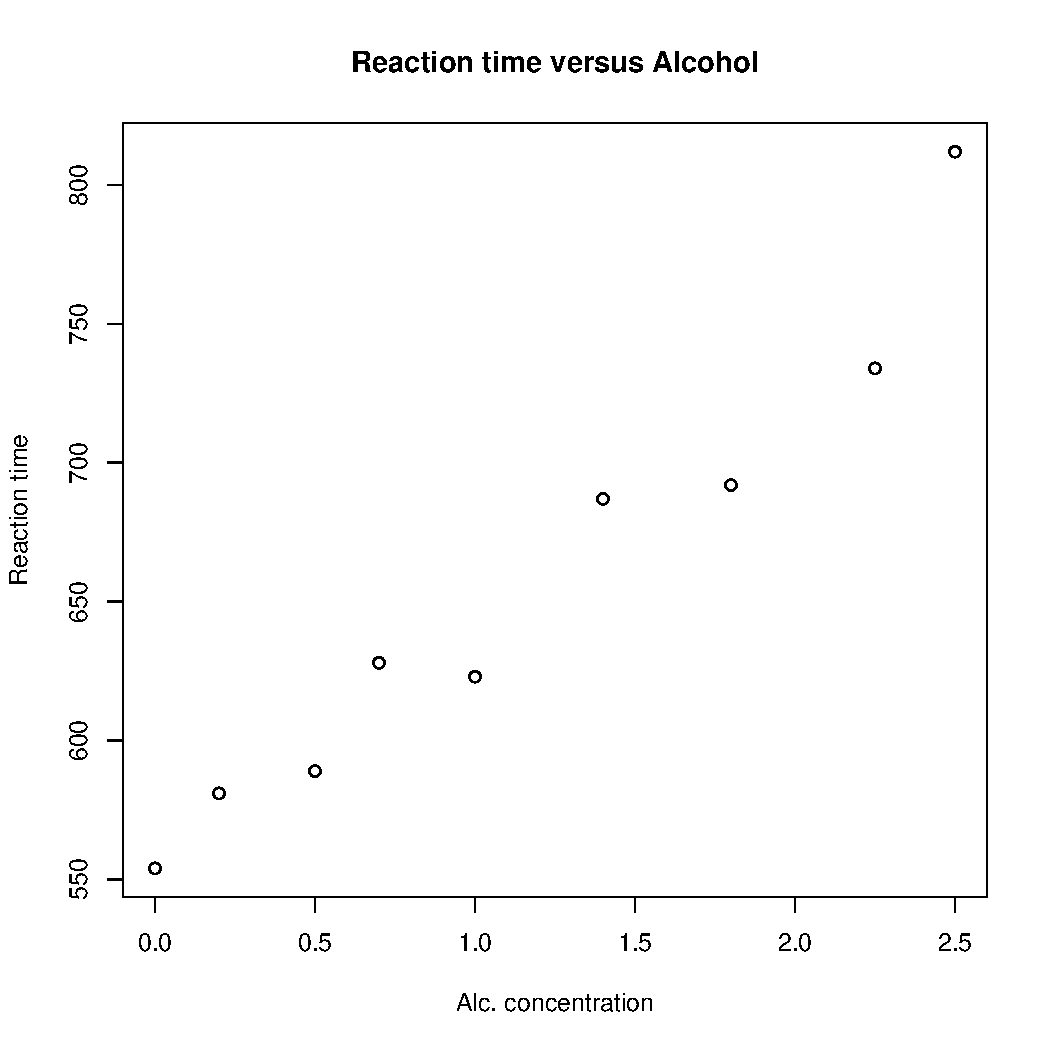
\includegraphics[width=.49\linewidth]{figures/unnamed-chunk-32-1} 

}



\end{knitrout}

\end{frame}

\begin{frame}[containsverbatim]
  \frametitle{built-in data \emph{women}}

\begin{knitrout}\tiny
\definecolor{shadecolor}{rgb}{0.973, 0.973, 0.973}\color{fgcolor}\begin{kframe}
\begin{alltt}
\hlstd{women}
\end{alltt}
\begin{verbatim}
##    height weight
## 1      58    115
## 2      59    117
## 3      60    120
## 4      61    123
## 5      62    126
## 6      63    129
## 7      64    132
## 8      65    135
## 9      66    139
## 10     67    142
## 11     68    146
## 12     69    150
## 13     70    154
## 14     71    159
## 15     72    164
\end{verbatim}
\end{kframe}
\end{knitrout}
  
\end{frame}


\begin{frame}[containsverbatim]
  \frametitle{\texttt{women\$height} and \texttt{women\$weight}}
  
\begin{knitrout}\tiny
\definecolor{shadecolor}{rgb}{0.973, 0.973, 0.973}\color{fgcolor}\begin{kframe}
\begin{alltt}
\hlkwd{plot}\hlstd{(women}\hlopt{$}\hlstd{height,women}\hlopt{$}\hlstd{weight,}\hlkwc{xlab}\hlstd{=}\hlstr{"height"}\hlstd{,}
     \hlkwc{ylab}\hlstd{=}\hlstr{"weight"}\hlstd{,}\hlkwc{main}\hlstd{=}\hlstr{"weight versus height"}\hlstd{)}
\end{alltt}
\end{kframe}

{\centering 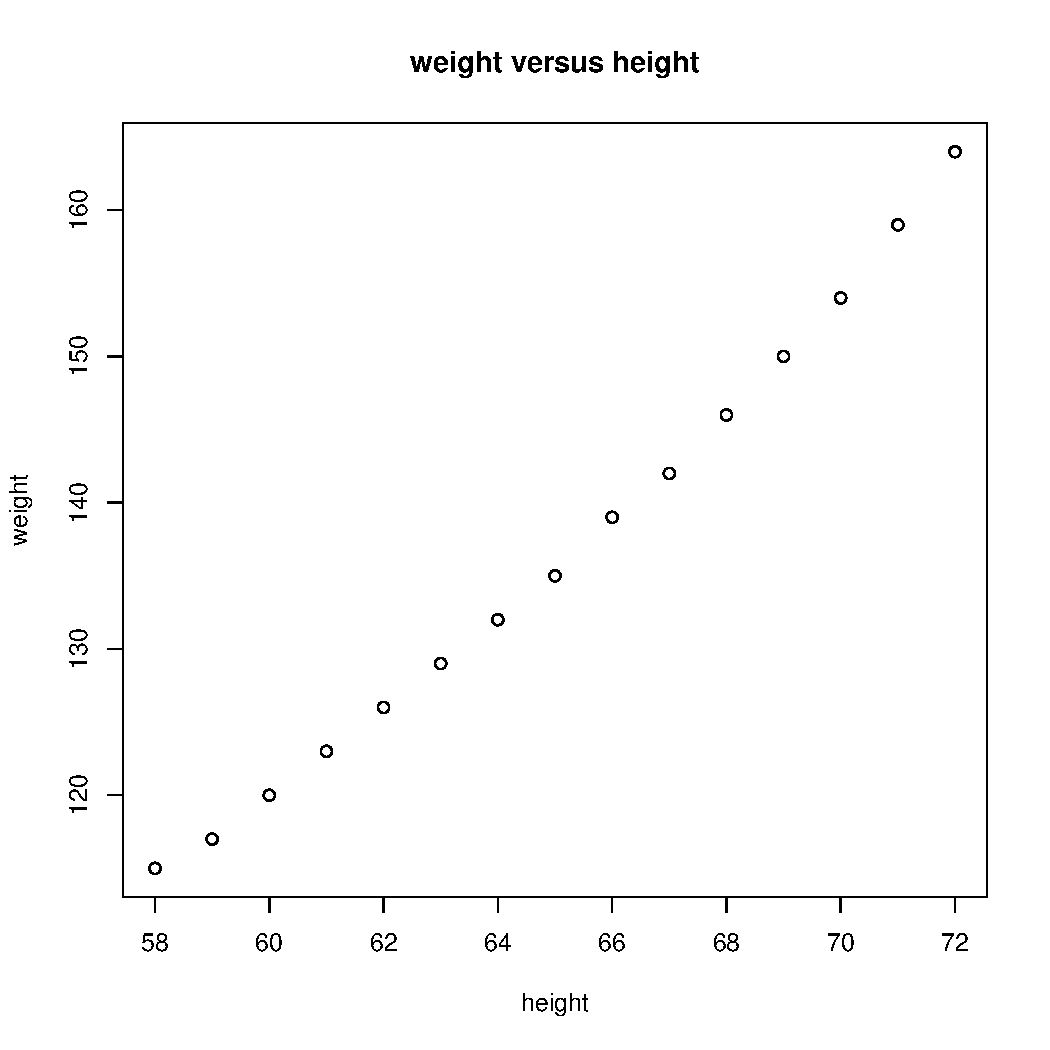
\includegraphics[width=.49\linewidth]{figures/unnamed-chunk-34-1} 

}



\end{knitrout}

\end{frame}

\begin{frame}[containsverbatim]
  \frametitle{Ausblick Schätzen und Testen:  \texttt{cor.test()}}
\small
\begin{knitrout}\tiny
\definecolor{shadecolor}{rgb}{0.973, 0.973, 0.973}\color{fgcolor}\begin{kframe}
\begin{alltt}
\hlkwd{cor}\hlstd{(women}\hlopt{$}\hlstd{height,women}\hlopt{$}\hlstd{weight,}\hlkwc{method}\hlstd{=}\hlstr{"pearson"}\hlstd{)}
\end{alltt}
\begin{verbatim}
## [1] 0.995
\end{verbatim}
\begin{alltt}
\hlkwd{cor.test}\hlstd{(women}\hlopt{$}\hlstd{height,women}\hlopt{$}\hlstd{weight)}
\end{alltt}
\begin{verbatim}
## 
## 	Pearson's product-moment correlation
## 
## data:  women$height and women$weight
## t = 38, df = 13, p-value = 1e-14
## alternative hypothesis: true correlation is not equal to 0
## 95 percent confidence interval:
##  0.986 0.999
## sample estimates:
##   cor 
## 0.995
\end{verbatim}
\end{kframe}
\end{knitrout}
  
\end{frame}


\begin{frame}[containsverbatim]
  \frametitle{More than two variables, \texttt{pairs()}}
\scriptsize
\begin{knitrout}\tiny
\definecolor{shadecolor}{rgb}{0.973, 0.973, 0.973}\color{fgcolor}\begin{kframe}
\begin{alltt}
\hlkwd{pairs}\hlstd{(swiss)}
\end{alltt}
\end{kframe}

{\centering 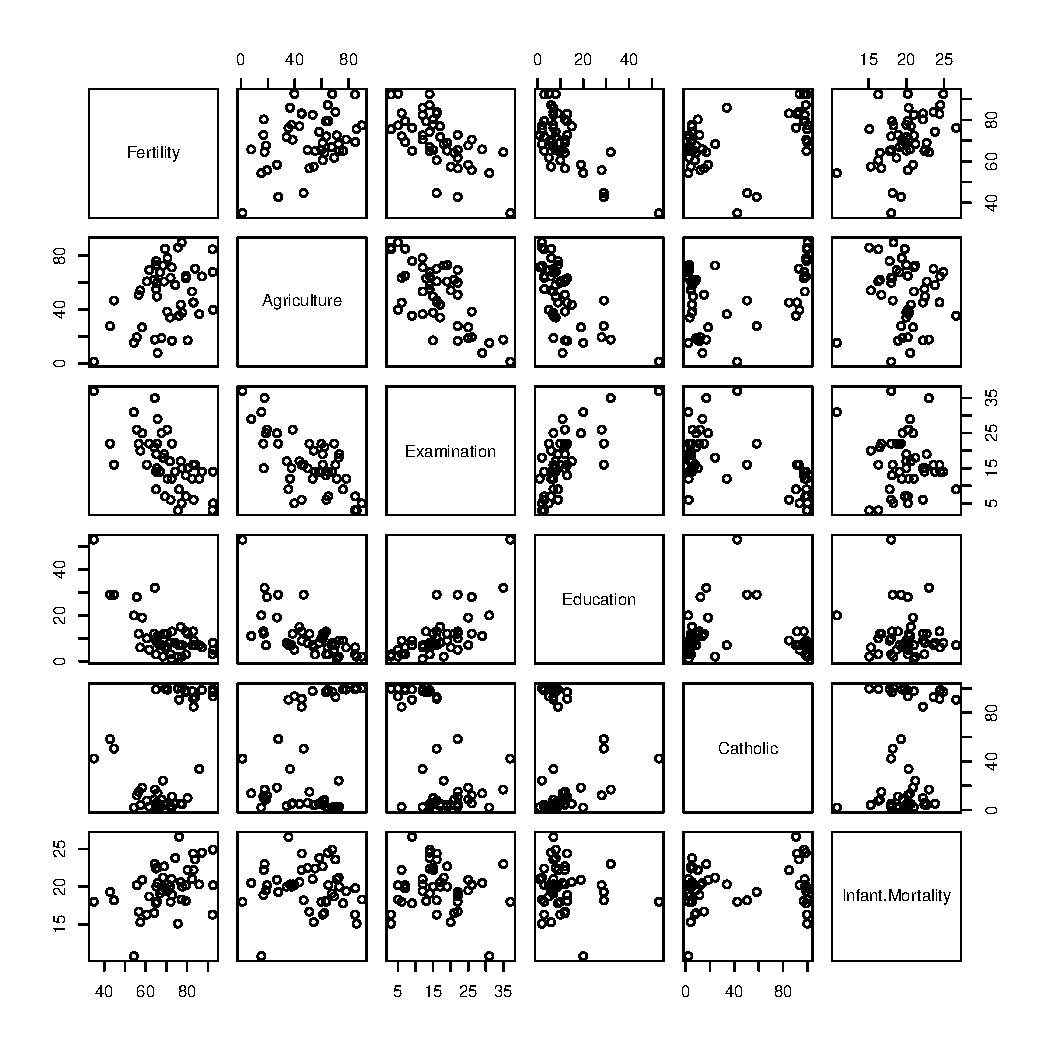
\includegraphics[width=.49\linewidth]{figures/unnamed-chunk-36-1} 

}



\end{knitrout}
  
\end{frame}



\begin{frame}
  \frametitle{Other correlation techniques}
  \begin{table}[h]
  \centering
  \begin{tabular}{lccc}\hline
    Y   /   X&intervall&ordinal&dichotom\\\hline
    \structure{intervall}&pearson&spearman &point-biserial\\
    \structure{ordinal}&spearman&spearman&biserial\\
    \structure{dichotom}&point-biserial&biserial&phi-coefficient\\\hline
  \end{tabular}
  \caption{correlation techniques}
  \label{tab: correlation techniques}
\end{table}
\end{frame}


\begin{frame}

\begin{knitrout}\tiny
\definecolor{shadecolor}{rgb}{0.973, 0.973, 0.973}\color{fgcolor}\begin{kframe}
\begin{alltt}
\hlkwd{citation}\hlstd{()}
\end{alltt}
\end{kframe}
\end{knitrout}

To cite R in publications use:

  R Development Core Team (2011). R: A language and environment for
  statistical computing. R Foundation for Statistical Computing,
  Vienna, Austria. ISBN 3-900051-07-0, URL http://www.R-project.org/.
  
\end{frame}



% \section{Bibliographie}




\begin{frame}
  \frametitle{Bibliographie}




\nocite{*}

%%add RcitePkgs if other packages
\bibliography{RcitePkgs,Rcite}  


\end{frame}




\end{document}







%%% Local Variables:
%%% mode: latex
%%% TeX-master: t
%%% End:
